\documentclass[conference]{IEEEtran}
\usepackage{amsmath,amssymb,amsfonts}
\usepackage{algorithmic}
\usepackage{algorithm}
\usepackage{graphicx}
\usepackage{textcomp}
\usepackage{xcolor}
\usepackage{booktabs}
\usepackage[turkish]{babel}
\usepackage[utf8]{inputenc}
\usepackage[T1]{fontenc}
\usepackage{cite}
\usepackage{url}

\begin{document}

\shorthandoff{=}
\shorthandoff{:}

\title{AutoLens AI: Görüntü İşleme ve Derin Öğrenme ile Araba Gövde Tipi Sınıflandırma}

\author{
\IEEEauthorblockN{Enes Demir}
\IEEEauthorblockA{\textit{Bilgisayar Mühendisliği} \\
\textit{Kocaeli Üniversitesi}\\
Kocaeli, Türkiye \\
230202066@kocaeli.edu.tr}
\and
\IEEEauthorblockN{Mert Şengül}
\IEEEauthorblockA{\textit{Bilgisayar Mühendisliği} \\
\textit{Kocaeli Üniversitesi}\\
Kocaeli, Türkiye \\
230202095@kocaeli.edu.tr}
}

\maketitle

\begin{abstract}
Sekiz farklı araba gövde tipini sınıflandırmak için AutoLens AI adlı derin öğrenme sistemi geliştirilmiştir. Sınıflar arası ciddi veri dengesizliği (Micro 22, SUV 670 örnek) Weighted Cross-Entropy Loss ile aşılmış; CNN ve Vision Transformer mimarileri sistematik olarak karşılaştırılmıştır. En yüksek başarım, öz-denetimli öğrenme ile ön eğitilmiş DINOv3 ViT-S/16 modelinin güvenli veri artırımı ve Dirichlet kalibrasyonu ile birleştirilmesiyle elde edilmiştir. Nihai model, 3170 örnekli iç test setinde \%95.99 doğruluk, 0.9537 Makro F1 ve \%0.97 Expected Calibration Error (ECE) değerlerine ulaşmıştır. Olasılık kalibrasyonunda Dirichlet yöntemi Temperature Scaling ve Vector Scaling'i Val NLL (0.1371), ECE (\%0.96) ve Test F1 (0.9537) metriklerinde geride bırakmıştır. Model 95 MB sınırının altında (82.6 MB ONNX) optimize edilmiş ve Gradio tabanlı web arayüzü ile sunulmuştur.
\end{abstract}

\begin{IEEEkeywords}
Derin Öğrenme, Görüntü Sınıflandırma, Vision Transformer, DINOv3, Kalibrasyon, Araba Gövde Tipi.
\end{IEEEkeywords}

\section{Giriş}
Günümüzde otonom sistemler, trafik yönetimi ve güvenlik alanlarında araçların fiziksel özelliklerinin doğru ve hızlı tespiti büyük önem taşımaktadır. Bu çalışma kapsamında, sekiz farklı araç gövde tipini (SUV, VAN, Station Wagon, Micro, Açık Tekerlekli/F1, Sedan, Hatchback, Pick-up) sınıflandırabilen bir derin öğrenme modeli geliştirilmiştir.

Katkılarımız dört ana başlıkta özetlenebilir:
\begin{enumerate}
\item \textbf{Sistematik model karşılaştırması:} Dört farklı mimari (ResNet18, EfficientNet-B2, MobileNetV4, DINOv3 ViT-S/16) aynı veri bölütlemesi ve değerlendirme protokolü altında karşılaştırılmış, LoRA ve tam ince ayar varyantları ayrı ayrı test edilmiştir. DINOv3'ün Makro F1'de CNN'lere +0.0183 ila +0.0682 puan üstünlük sağladığı gösterilmiştir.
\item \textbf{Veri dengesizliği stratejisi:} Focal Loss ($\gamma=2.0$) ve Weighted Cross-Entropy Loss (maksimum ağırlık 5.0), DINOv3 üzerinde ablasyon çalışmalarıyla karşılaştırılmış; Weighted CE'nin Makro F1'de +0.0205, azınlık sınıflarında ise +0.065'e varan üstünlük sağladığı deneysel olarak kanıtlanmıştır.
\item \textbf{Güvenli veri artırımı (safe augmentation):} Aracın siluetini koruyan, agresif geometrik dönüşümlerden kaçınan bir artırım politikası uygulanmış ve EMA (Exponential Moving Average) ile birleştirildiğinde Makro F1'de +0.0320 puanlık iyileşme sağlanmıştır.
\item \textbf{Kapsamlı olasılık kalibrasyonu:} Temperature Scaling, Vector Scaling ve Dirichlet (ODIR) yöntemleri grid search ile karşılaştırılmış; Dirichlet kalibrasyonu ile ECE \%10.33'ten \%0.96'ya düşürülerek modelin aşırı güven (overconfidence) sorunu giderilmiştir. Ayrıca farklı modellerin (EfficientNet-B2, DINOv3 baseline) kalibrasyon ihtiyaçları analiz edilmiştir.
\end{enumerate}

Veri seti Kaggle ve Hugging Face üzerinde yayımlanmış açık veri kümelerinden toplanmış, sınıflar arası dengesizlik sınıf ağırlıklı hata fonksiyonları ile ele alınmıştır. Proje teslim gereksinimleri doğrultusunda model 95 MB altında ONNX formatında paketlenmiş ve canlı demo web arayüzü ile sunulmuştur.

\section{İlgili Çalışmalar}
Araç tipi sınıflandırma literatürü, el yapımı özniteliklerden derin öğrenme tabanlı temsillere doğru belirgin bir dönüşüm geçirmiştir. Dong ve arkadaşları, önden görünüşlü araç görüntüleri için yarı denetimli bir CNN önermiş ve 9850 yüksek çözünürlüklü örnekten oluşan BIT-Vehicle veri seti üzerinde araç tipi sınıflandırmasını incelemiştir \cite{dong2015vehicle}. Bu çalışma, sınırlı etiketli veri koşullarında dahi evrişimsel temsillerin HOG, SIFT ve Gabor gibi el yapımı özniteliklere kıyasla daha ayırt edici olabildiğini göstermesi bakımından önemlidir. Krause ve arkadaşlarının Stanford Cars veri seti ise 197 araç kategorisi ve 16185 görüntüyle ince taneli araç tanıma problemini model, yıl ve gövde benzerliği gibi daha zor ayrımlara taşımıştır \cite{krause2013cars}. Gebru ve arkadaşları 50 milyon sokak görünümü görüntüsünden 22 milyon aracı algılayıp marka, model, yıl ve gövde tipi gibi nitelikleri tahmin ederek araç sınıflandırmasının yalnızca trafik sistemlerinde değil, büyük ölçekli görsel analitikte de kullanılabileceğini göstermiştir \cite{gebru2017streetview}.

Güncel çalışmalar, araç sınıflandırmasını algılama, takip ve karar destek bileşenleriyle birlikte ele almaktadır. Kim, DashCam görüntülerinde YOLO tabanlı araç algılama ve ResNet-50 aktarım öğrenmesi ile araç tipini dört, rengini sekiz sınıfta sınıflandıran bir sistem önermiş; araç tipi sınıflandırmasında \%93.9 doğruluk bildirmiştir \cite{kim2024vehicle}. Bu yaklaşım, gerçek zamanlı sürüş senaryolarında araç tipinin güvenlik kararları için doğrudan kullanılabileceğini göstermektedir. AutoLens AI ise bu çizgiyi, kameralı trafik algılamasından farklı olarak yüklenen tekil araç görüntülerinde sekiz gövde tipini ayırt etmeye ve özellikle Hatchback--Sedan, Pick-up--SUV gibi morfolojik olarak yakın sınıfları ayrıştırmaya odaklamaktadır.

Görüntü sınıflandırmada ResNet, artık bağlantılar sayesinde derin ağların optimize edilmesini kolaylaştırmış; EfficientNet ise derinlik, genişlik ve çözünürlüğü birlikte ölçekleyen compound scaling yaklaşımıyla doğruluk/verimlilik dengesini iyileştirmiştir \cite{he2016deep,tan2019efficientnet}. Mobil çıkarım tarafında MobileNetV4, Universal Inverted Bottleneck bloğu ve mobil dikkat mekanizmalarıyla farklı hızlandırıcılar üzerinde Pareto-verimli mimariler önermektedir \cite{qin2024mobilenetv4}. Bu nedenle AutoLens AI'da CNN adayları yalnızca temel karşılaştırma noktaları değil, aynı zamanda model boyutu ve çıkarım maliyeti açısından da anlamlı basamaklar olarak değerlendirilmiştir.

Transformer tabanlı görüntü modelleri, görüntüyü yama dizisi olarak işleyerek küresel bağlamsal ilişkileri doğrudan modelleyebilmekte ve CNN'lerin yerel alıcı alan sınırlamasını azaltmaktadır \cite{dosovitskiy2020image}. DINO ve DINOv2, etiket kullanmadan öğrenilen öz-denetimli görsel temsillerin nesne bölütleme, sınıflandırma ve aktarım öğrenmesinde güçlü özellikler üretebildiğini göstermiştir \cite{caron2021emerging,oquab2023dinov2}. DINOv3 ise ölçeklenmiş veri hazırlığı, Gram anchoring ve çözünürlük uyarlama stratejileriyle yoğun özellik kalitesini artıran daha güncel bir görsel temel model ailesi sunmaktadır \cite{simeoni2025dinov3}. Bu bağlamda DINOv3'ün AutoLens AI için seçilmesi, sınırlı ve dengesiz etiketli veri altında önceden öğrenilmiş genel görsel temsillerden yararlanma motivasyonuna dayanmaktadır.

Dengesiz sınıf dağılımı ve olasılık kalibrasyonu, bu çalışmanın metodolojik eksenini oluşturan iki tamamlayıcı problemdir. Focal Loss, yoğun algılama görevlerinde kolay örneklerin etkisini azaltıp zor örneklere odaklanmak için önerilmiş ve sınıf dengesizliği literatüründe yaygın bir referans haline gelmiştir \cite{lin2017focal}. Öte yandan modern derin ağların yüksek doğruluğa rağmen zayıf kalibre olabildiği, Guo ve arkadaşları tarafından ayrıntılı biçimde gösterilmiş; Temperature Scaling pratik ve güçlü bir sonradan kalibrasyon yöntemi olarak öne çıkarılmıştır \cite{guo2017calibration}. Kull ve arkadaşlarının Dirichlet kalibrasyonu ise çok sınıflı olasılık vektörlerinde Temperature Scaling'in tek parametreli yapısına kıyasla daha esnek bir düzeltme sunmaktadır \cite{kull2019beyond}. AutoLens AI'daki Weighted Cross-Entropy, Focal Loss ve Dirichlet kalibrasyonu karşılaştırmaları bu literatürdeki bulguları araç gövde tipi sınıflandırması bağlamında deneysel olarak sınamaktadır.

\section{Sistem Mimarisi ve Metodoloji}

\subsection{Veri Seti ve Ön İşleme}

\begin{table}[h]
\centering
\small
\caption{Test seti sınıf dağılımları (3170 örnek)}
\label{tab:dataset_dist}
\begin{tabular}{@{}lrr@{}}
\toprule
\textbf{Sınıf} & \textbf{Örnek Sayısı} & \textbf{Oran (\%)} \\ \midrule
Sedan & 836 & 26.4 \\
SUV & 670 & 21.1 \\
Açık Tekerlekli (F1) & 586 & 18.5 \\
VAN & 455 & 14.4 \\
Pick Up & 269 & 8.5 \\
Hatchback & 266 & 8.4 \\
Station Wagon & 66 & 2.1 \\
Micro & 22 & 0.7 \\ \bottomrule
\end{tabular}
\end{table}
Sınıflandırma için SUV, VAN, Station Wagon, Micro, Açık Tekerlekli (F1), Sedan, Hatchback ve Pick Up olmak üzere 8 sınıf belirlenmiştir. Toplam 31,612 görüntü Kaggle ve Hugging Face kaynaklı açık veri kümelerinden toplanmış, hedef sınıf tanımlarıyla uyumlu olacak şekilde yeniden etiketlenmiş ve iki aşamalı tabakalı (stratified) rastgele bölme ile ayrılmıştır. Kaynak veri kümeleri doğrudan tek bir sınıflandırma problemi olarak kullanılmamış; yalnızca hedef 8 sınıfa güvenilir biçimde eşlenebilen örnekler seçilmiştir (Tablo \ref{tab:source_datasets}).

\begin{table*}[t]
\centering
\footnotesize
\caption{Özelleştirilmiş veri setini oluşturan açık kaynak veri kümeleri}
\label{tab:source_datasets}
\begin{tabular}{@{}p{0.26\textwidth}p{0.12\textwidth}rp{0.44\textwidth}@{}}
\toprule
\textbf{Kaynak} & \textbf{Platform} & \textbf{Kullanılan} & \textbf{Katkı} \\ \midrule
Cars Body Type Cropped \cite{dataset_cars_body_type_cropped} & Kaggle & 5,370 & Hatchback, Pick Up, SUV, Sedan, VAN \\
Stanford Cars by Classes Folder \cite{krause2013cars,dataset_stanford_cars_folder} & Kaggle & 10,928 & Temel araç sınıfları ve Micro örnekleri \\
Vehicle Classification Dataset \cite{dataset_vehicle_classification_ihasib} & Kaggle & 1,843 & Hatchback, Sedan, SUV, Pick Up \\
Vehicle Images Dataset \cite{dataset_vehicle_images_lyensoetanto} & Kaggle & 6,612 & Sedan, SUV, VAN \\
VehicleType-10 \cite{competition_vehicletype10} & Kaggle & 488 & Ek gövde tipi çeşitliliği \\
F1 Image Classification Updated \cite{dataset_f1_updated} & Kaggle & 5,846 & Açık tekerlekli/F1 sınıfı \\
CBSC \cite{dataset_cbsc_hf} & Hugging Face & 325 & Küçük ölçekli gövde tipi doğrulaması \\
Vehicle Classification \cite{dataset_drbimmer_hf} & Hugging Face & 200 & VAN sınıfı desteği \\ \bottomrule
\end{tabular}
\end{table*}

Bu kaynaklar, proje dokümanında özellikle vurgulanan ``Kaggle, Hugging Face vb. çeşitli kaynaklardan ham görsel toplayarak özelleştirilmiş veri seti oluşturma'' gereksinimini karşılamaktadır. Her kaynak için ham etiket, dönüştürülmüş hedef etiket, kabul/ret gerekçesi ve lisans notu kayıt altına alınmıştır. Convertible, coupe, bus, truck ve cabriolet gibi hedef 8 sınıfta karşılığı bulunmayan veya morfolojik olarak belirsiz örnekler eğitimden çıkarılmış; böylece modelin değerlendirmesi yalnızca teslimde beklenen sınıflar üzerinde yapılmıştır.

\begin{equation}
S_{\text{eligible}} \xrightarrow[\text{stratify}]{80\%} S_{\text{train}} \;,\quad 
S_{\text{remain}} \xrightarrow[\text{stratify}]{50\%} S_{\text{val}} + S_{\text{test}}
\label{eq:split}
\end{equation}

Veri seti iki aşamalı ve tabakalı bir protokolle ayrılmıştır. İlk aşamada örneklerin $\%80$'i eğitim kümesine (25,285) alınmış, kalan $\%20$'lik bölüm ikinci aşamada eşit biçimde doğrulama (3,157) ve iç test (3,170) kümelerine bölünmüştür. Tabakalı bölme sayesinde her sınıfın eğitim/doğrulama/test setlerindeki oranı korunmuştur (Tablo \ref{tab:split_dist}).

\begin{table}[h]
\centering
\small
\caption{Sınıfların eğitim/doğrulama/iç test dağılımı}
\label{tab:split_dist}
\begin{tabular}{@{}lrrr@{}}
\toprule
\textbf{Sınıf} & \textbf{Eğitim} & \textbf{Doğrulama} & \textbf{İç Test} \\ \midrule
Sedan       & 6,680 & 835 & 836 \\
SUV         & 5,351 & 668 & 670 \\
F1          & 4,676 & 584 & 586 \\
VAN         & 3,631 & 453 & 455 \\
Hatchback   & 2,120 & 265 & 266 \\
Pick Up     & 2,143 & 267 & 269 \\
St. Wagon   & 520   & 65  & 66  \\
Micro       & 164   & 20  & 22  \\ \midrule
\textbf{Toplam} & \textbf{25,285} & \textbf{3,157} & \textbf{3,170} \\ \bottomrule
\end{tabular}
\end{table}

Sınıf dağılımları doğal olarak dengesizdir: en büyük sınıf Sedan (836 test örneği) ile en küçük sınıf Micro (22 test örneği) arasında yaklaşık 38 kat fark bulunmaktadır. Ön işleme aşamasında bozuk/uygunsuz dosyalar elenmiş, kabul edilen görüntüler RGB biçimine çevrilmiş, DINOv3 için $256\times256$ boyutunda yeniden boyutlandırılıp merkez kırpma uygulanmış ve tensörler ImageNet ortalama/standart sapma değerleriyle normalize edilmiştir. CNN karşılaştırma modellerinde aynı protokol $224\times224$ giriş boyutu ile uygulanmıştır.

Veri artırımı (data augmentation) politikası dikkatle tasarlanmıştır. Amaç, modelin genelleme kapasitesini artırırken aracın ayırt edici siluet özelliklerini korumaktır. Bu nedenle ``güvenli'' bir artırım politikası benimsenmiştir. Bu politika; rastgele yatay çevirme, hafif perspektif değişimi, sınırlı parlaklık/kontrast/doygunluk düzenlemesi, düşük düzeyli bulanıklaştırma ve yerel kontrast iyileştirme adımlarından oluşmaktadır. Hatchback-Sedan ayrımını bozacak agresif kırpma, döndürme veya esnetmeden kaçınılmıştır. Böylece modelin gerçek dünya varyasyonlarına karşı dayanıklılığını artırırken sınıflar arası ayrımı zorlaştıracak artefaktlardan kaçınmak hedeflenmiştir.

\subsection{Model Mimarisi ve Karşılaştırması}

\subsubsection{CNN Modelleri}
İlk aşamada üç CNN mimarisi ImageNet ön eğitimi ile tam ince ayar (full fine-tune) yapılarak değerlendirilmiştir: 

\textbf{ResNet18} (11.2M parametre): Artık bağlantıları (residual connections) sayesinde 18 katmanlı derin ağ eğitimini kolaylaştıran temel CNN mimarisidir \cite{he2016deep}. 512 boyutlu öznitelik vektörü ile sınıflandırma katmanına bağlanmıştır. Düşük parametre sayısı sayesinde hızlı eğitim ve çıkarım avantajı sunmaktadır.

\textbf{EfficientNet-B2} (9.0M parametre): Compound scaling prensibi ile derinlik, genişlik ve çözünürlüğü birlikte optimize eden verimli bir mimaridir \cite{tan2019efficientnet}. B2 varyantı, 140$\times$140 taban çözünürlük ve 1.1 derinlik katsayısı ile dengeli bir performans sunmaktadır. B0'a kıyasla daha yüksek kapasiteye sahiptir.

\textbf{MobileNetV4-Conv-M} (9.0M parametre): 2024 yılında yayımlanan, mobil cihazlarda çıkarım için tasarlanmış güncel bir CNN modelidir \cite{qin2024mobilenetv4}. Universal Inverted Bottleneck (UIB) bloğu ile hem konvansiyonel hem de mobil-optimize edilmiş operasyonları birleştirmektedir.

Tüm CNN'ler 30 epoch boyunca eğitilmiş, öğrenme oranı 0.001 ve 128 örneklik mini-batch kullanılmıştır. Erken durdurma ve en iyi model seçimi doğrulama F1 skoruna göre yapılmıştır.

\subsubsection{Vision Transformer: DINOv3}
CNN'lerin ardından Vision Transformer tabanlı \textbf{DINOv3 ViT-S/16} (21.6M parametre) değerlendirilmiştir. DINOv3, Meta AI tarafından geliştirilen üçüncü nesil DINO serisi olup ImageNet-1K üzerinde öz-denetimli öğrenme (self-supervised learning) ile ön eğitilmiştir \cite{simeoni2025dinov3}. ViT-S/16 varyantı, 16$\times$16 piksel boyutunda görüntü parçacıkları (patch) kullanan 21.6M parametreli küçük bir Vision Transformer'dır \cite{dosovitskiy2020image}. Öz-denetimli eğitim sayesinde etiketli veriye ihtiyaç duymadan güçlü görsel temsiller öğrenmekte ve transfer öğrenmede yüksek başarım sağlamaktadır.

İki ince ayar stratejisi test edilmiştir: (1) \textbf{Full fine-tune (tam ince ayar)} -- tüm model ağırlıkları güncellenmiş, yeni sınıflara tam uyum sağlanmıştır. (2) \textbf{LoRA} (Low-Rank Adaptation) -- yalnızca 0.3M ek parametreyle düşük ranklı adaptasyon denenmiştir \cite{hu2022lora}. LoRA, büyük modellerde parametre verimli ince ayar için popüler bir yöntem olmasına rağmen, bu çalışmada beklentiyi karşılamamıştır.

\begin{table}[h]
\centering
\small
\caption{Aday modellerin mimari karşılaştırması}
\label{tab:arch_sizes}
\begin{tabular}{@{}lrrr@{}}
\toprule
\textbf{Model} & \textbf{Parametre} & \textbf{Giriş} & \textbf{ONNX} \\ \midrule
DINOv3 ViT-S/16 & 21.6M & $256^2$ & 82.6 MB \\
ResNet18         & 11.2M & $224^2$ & 42.6 MB \\
EfficientNet-B2  &  9.0M & $224^2$ & 29.4 MB \\
MobileNetV4      &  9.0M & $224^2$ & 32.1 MB \\ \bottomrule
\end{tabular}
\end{table}

\begin{table}[h]
\centering
\scriptsize
\caption{Tüm model adaylarının iç test karşılaştırması (3170 örnek)}
\label{tab:model_comparison}
\begin{tabular}{@{}lccc@{}}
\toprule
\textbf{Model} & \textbf{Acc. $\uparrow$} & \textbf{Macro F1 $\uparrow$} & \textbf{W. F1 $\uparrow$} \\ \midrule
\textbf{DINOv3 Full} & \textbf{0.9438} & \textbf{0.9187} & \textbf{0.9442} \\
EfficientNet-B2 & 0.9205 & 0.9004 & 0.9205 \\
ResNet18 & 0.8968 & 0.8583 & 0.8963 \\
MobileNetV4 & 0.8899 & 0.8505 & 0.8905 \\
DINOv3 LoRA & 0.7820 & 0.6316 & -- \\ \bottomrule
\end{tabular}
\end{table}

İç test seti sonuçları (Tablo \ref{tab:model_comparison}) incelendiğinde, DINOv3 full fine-tune varyantı tüm metriklerde CNN tabanlı modelleri geride bırakmıştır. EfficientNet-B2, CNN'ler arasında en başarılı model olurken (0.9004 Macro F1), MobileNetV4 en düşük performansı göstermiştir (0.8505). DINOv3'ün LoRA varyantı 0.6316 Macro F1 ile beklentinin altında kalmış ve elenmiştir. DINOv3'ün öz-denetimli ön eğitimi sayesinde sınırlı veri ile yüksek genelleme sağladığı, özellikle Macro Recall'de (0.9121) CNN'lere belirgin üstünlük kurduğu gözlemlenmiştir.

DINOv3'ün CNN'lere üstünlüğünün temel nedeni, öz-denetimli (self-supervised) ön eğitim sırasında ImageNet üzerinde etiket kullanmadan öğrenilen zengin görsel temsillerdir. ViT mimarisi, global attention mekanizması sayesinde bir aracın tüm gövde yapısını bütüncül olarak değerlendirebilmekte, CNN'lerin yerel reseptif alan sınırlamasını aşmaktadır. EfficientNet-B2'nin CNN'ler arasında öne çıkması, compound scaling stratejisinin dengeli bir öznitelik çıkarıcı sağlamasıyla açıklanabilir. LoRA'nın başarısızlığı ise düşük ranklı adaptasyonun DINOv3 gibi öz-denetimli bir modelin temsil uzayını yeni sınıflara yeterince uyarlayamamasından kaynaklanmaktadır: yalnızca 0.3M parametre (toplamın \%1.4'ü) güncellenmiş, bu da görev odaklı ince ayar için yetersiz kalmıştır.

\subsection{Eğitim Süreci ve Hiperparametre Seçimi}
Nihai model mimarisi DINOv3 olarak belirlendikten sonra eğitim hiperparametreleri deneysel olarak optimize edilmiştir. AdamW optimizörü, $\beta_1=0.9$, $\beta_2=0.999$ varsayılan parametreleriyle kullanılmış; öğrenme oranı 0.0001, weight decay 0.0001 olarak ayarlanmıştır \cite{loshchilov2019adamw}. Öğrenme oranı seçiminde, Vision Transformer modelleri için önerilen düşük öğrenme oranı stratejisi izlenmiş; Cosinus Annealing yerine sabit öğrenme oranı tercih edilmiştir.

Label smoothing ($\varepsilon=0.05$) kaybı aşağıdaki gibi düzenlemektedir:
\begin{equation}
\mathcal{L}_{\text{LS}} = -(1-\varepsilon) \log(p_y) - \frac{\varepsilon}{K} \sum_{k=1}^{K} \log(p_k)
\end{equation}
Burada $K=8$ sınıf sayısı, $p_y$ doğru sınıf olasılığıdır. Label smoothing, modelin aşırı güvenli tahminler yapmasını engelleyerek genelleme kapasitesini artırmakta ve kalibrasyonu iyileştirmektedir \cite{szegedy2016inception}. Ön denemelerde $\varepsilon=0.1$ ile kalibrasyon sonrası ECE'de \%0.2 mutlak iyileşme gözlemlenmiş ancak F1'de hafif düşüş yaşanmış; $\varepsilon=0.05$ denge noktası olarak seçilmiştir.

Drop path rate (0.1) ve weight decay (0.0001) ek düzenlileştirme sağlamaktadır. EMA (Exponential Moving Average, decay=0.999) ile her adımda model ağırlıklarının yumuşatılmış ortalaması alınmış, $\theta_{\text{EMA}} \leftarrow 0.999 \cdot \theta_{\text{EMA}} + 0.001 \cdot \theta$ şeklinde güncellenmiştir. Gradient clipping (max norm=1.0) ile gradyan patlaması önlenmiştir. Erken durdurma, doğrulama kümesindeki makro F1 başarımı temel alınarak uygulanmış; eğitim 42. epoch sonunda durdurulmuş, en iyi ağırlıklar 29. epoch'tan seçilmiştir.

\subsection{Ablasyon Çalışmaları}

\subsubsection{Kayıp Fonksiyonu: Focal vs Weighted CE}
Sınıf dengesizliğini ele almak için iki kayıp fonksiyonu DINOv3 üzerinde karşılaştırılmıştır. Weighted Cross-Entropy, her örnek için sınıf frekansının tersiyle ağırlıklandırma yaparken (maksimum ağırlık 5.0 ile sınırlı), Focal Loss ($\gamma=2.0$) kolay örneklerin katkısını azaltarak zor örneklere odaklanmaktadır \cite{lin2017focal}. Matematiksel olarak:

\begin{equation}
\mathcal{L}_{\text{WCE}} = -\frac{1}{N} \sum_{i=1}^{N} w_{y_i} \log(p_{i,y_i}), \quad
w_c = \min\!\left(\frac{N}{K \cdot n_c},\, 5.0\right)
\label{eq:wce}
\end{equation}

\begin{equation}
\mathcal{L}_{\text{Focal}} = -\frac{1}{N} \sum_{i=1}^{N} (1 - p_{i,y_i})^\gamma \log(p_{i,y_i})
\label{eq:focal}
\end{equation}

Burada $N$ toplam örnek, $K=8$ sınıf, $n_c$ sınıf $c$'nin frekansı, $p_{i,y_i}$ $i$ örneğinin doğru sınıf olasılığıdır. Her iki model aynı veri artırımı ve EMA politikası ile eğitilmiştir. Weighted CE'de ağırlık tavanı (clipping) 5.0 ile sınırlanarak aşırı ağırlıklandırmanın gürültü amplifikasyonu engellenmiştir.

\begin{table}[h]
\centering
\caption{Kayıp Fonksiyonu Ablasyonu -- İç Test Seti Genel Metrikler (DINOv3 + Safe Aug + EMA)}
\label{tab:loss_ablation}
\begin{tabular}{@{}lccc@{}}
\toprule
\textbf{Metric} & \textbf{Weighted CE} & \textbf{Focal Loss} & \textbf{Fark} \\ \midrule
Accuracy $\uparrow$ & \textbf{0.9584} & 0.9505 & +0.0079 \\
Macro F1 $\uparrow$ & \textbf{0.9507} & 0.9302 & +0.0205 \\
Weighted F1 $\uparrow$ & \textbf{0.9584} & 0.9502 & +0.0082 \\
Macro Precision $\uparrow$ & \textbf{0.9561} & 0.9358 & +0.0203 \\
Macro Recall $\uparrow$ & \textbf{0.9456} & 0.9269 & +0.0187 \\ \bottomrule
\end{tabular}
\end{table}

İç test setinde Weighted CE, tüm metriklerde Focal Loss'a üstünlük sağlamıştır. En büyük fark Makro F1'de (+0.0205) görülmüştür. Focal Loss'un iyi öğrenilmiş sınıflardaki kaybı sıfıra yaklaştırma özelliği, dengeli sınıflarda avantaj sağlasa da azınlık sınıflarındaki zayıf performansı genel başarımı düşürmüştür.

\begin{table}[h]
\centering
\caption{Sınıf Bazlı F1 Karşılaştırması: Weighted CE vs Focal Loss (İç Test Seti)}
\label{tab:class_f1_comparison}
\begin{tabular}{@{}lccc@{}}
\toprule
\textbf{Sınıf} & \textbf{Weighted CE F1 $\uparrow$} & \textbf{Focal Loss F1 $\uparrow$} & \textbf{Fark} \\ \midrule
SUV & \textbf{0.9504} & 0.9372 & +0.0132 \\
VAN & \textbf{0.9856} & 0.9832 & +0.0024 \\
Station Wagon & \textbf{0.9302} & 0.8652 & \textbf{+0.0650} \\
Micro & \textbf{0.9767} & 0.9302 & \textbf{+0.0465} \\
F1 & \textbf{0.9991} & 0.9966 & +0.0025 \\
Sedan & \textbf{0.9591} & 0.9589 & +0.0002 \\
Hatchback & \textbf{0.8731} & 0.8628 & +0.0103 \\
Pick Up & \textbf{0.9314} & 0.9070 & +0.0244 \\ \bottomrule
\end{tabular}
\end{table}

Tablo \ref{tab:class_f1_comparison} sınıf bazlı detay incelendiğinde, Weighted CE'nin özellikle azınlık sınıflarında (Micro +0.0465, Station Wagon +0.0650, Pick Up +0.0244) belirgin iyileşme sağladığı görülmektedir. Bol örnekli sınıflarda (Sedan, VAN, F1) iki yöntem arasındaki fark ihmal edilebilir düzeydedir. Bu sonuç, ağırlıklandırma stratejisinin dengesiz veri setlerinde Focal Loss'a kıyasla daha etkili olduğunu göstermektedir.

\subsubsection{Veri Artırımı Etkisi}
Veri artırımının katkısını ölçmek için augmentasyonsuz DINOv3 (Baseline) ile safe augmentation + EMA kullanılan versiyon karşılaştırılmıştır:

\begin{table}[h]
\centering
\scriptsize
\caption{Veri artırımı ablasyonu (DINOv3 + Weighted CE, iç test)}
\label{tab:aug_ablation}
\begin{tabular}{@{}lccc@{}}
\toprule
\textbf{Konfig.} & \textbf{Acc. $\uparrow$} & \textbf{Macro F1 $\uparrow$} & \textbf{W. F1 $\uparrow$} \\ \midrule
Baseline & 0.9438 & 0.9187 & 0.9442 \\
Safe Aug + EMA & \textbf{0.9584} & \textbf{0.9507} & \textbf{0.9584} \\ \bottomrule
\end{tabular}
\end{table}

İç test setinde safe augmentation ve EMA eklenmesi tüm metriklerde iyileşme sağlamış, Makro F1'de +0.0320 puanlık bir artış elde edilmiştir. Bu iyileşmenin büyük kısmı, veri artırımının özellikle az örnekli sınıflardaki genelleme kapasitesini artırmasından kaynaklanmaktadır.

\subsection{Olasılık Kalibrasyonu}

\subsubsection{Kalibrasyon Problemi ve Yöntemler}
Derin öğrenme modelleri genellikle aşırı güven (overconfidence) eğilimindedir: bir görüntüyü \%90 olasılıkla sınıflandırdıklarında, gerçek doğruluk oranı \%90'ın altında olabilir \cite{guo2017calibration}. Bu çalışmada üç kalibrasyon yöntemi karşılaştırılmıştır:

\textbf{Temperature Scaling:} Softmax çıktılarına tek bir sıcaklık parametresi ($T$) uygulayarak olasılıkları yumuşatır: $\hat{p}_k = \sigma_{\text{SM}}(\mathbf{z}/T)_k$. Tek parametreli olduğu için en basit yöntemdir ancak her sınıf için aynı düzeltmeyi uygular \cite{guo2017calibration}. $T=1.0$ kalibrasyonsuz duruma, $T>1$ daha düz (uniform) olasılıklara, $T<1$ daha keskin olasılıklara karşılık gelir.

\textbf{Vector Scaling:} Her sınıf için ayrı bir ağırlık vektörü ($\mathbf{w}$) ve bias ($b$) öğrenir: $\hat{p}_k = \sigma_{\text{SM}}(\mathbf{w} \odot \mathbf{z} + \mathbf{b})_k$. Temperature Scaling'den daha esnektir ancak aşırı öğrenmeye yatkındır; bu nedenle L2 düzenlileştirme ($\lambda$) ile birlikte kullanılır.

\textbf{Dirichlet (ODIR) Kalibrasyonu:} Her sınıf için ayrı bir beta dağılımı parametrelendirerek sınıf bazlı olasılık düzeltmesi yapar (\cite{kull2019beyond}). ODIR (Ordered Dirichlet) versiyonu, sınıf sıralamasını koruyarak daha kararlı kalibrasyon sağlar.

\subsubsection{DINOv3 Weighted Kalibrasyon Sonuçları}
DINOv3 Weighted modeli üzerinde tüm yöntemler grid search ile optimize edilmiştir. Dirichlet ve Vector Scaling için $\lambda \in \{0.001, 0.01, 0.1, 1.0\}$ değerleri taranmıştır.

\begin{table}[h]
\centering
\caption{Kalibrasyon Yöntemleri Karşılaştırması (DINOv3 Weighted, Doğrulama/Test)}
\label{tab:calibration}
\begin{tabular}{@{}lccc@{}}
\toprule
\textbf{Yöntem} & \textbf{Val NLL $\downarrow$} & \textbf{ECE $\downarrow$} & \textbf{Test F1} \\ \midrule
Kalibrasyonsuz & 0.2585 & 0.1033 & -- \\
Temperature Scaling & 0.2045 & 0.0211 & 0.9496 \\
Vector Scaling ($\lambda=0.01$) & 0.1706 & 0.0232 & 0.9450 \\
\textbf{Dirichlet ($\lambda=0.001$)} & \textbf{0.1371} & \textbf{0.0096} & \textbf{0.9537} \\ \bottomrule
\end{tabular}
\end{table}

\begin{table}[h]
\centering
\caption{İç Test Seti Kalibrasyon Metrikleri (DINOv3 Weighted)}
\label{tab:calibration_detail}
\begin{tabular}{@{}lcccc@{}}
\toprule
\textbf{Metrik} & \textbf{Öncesi} & \textbf{Temp.} & \textbf{Vector} & \textbf{Dirichlet} \\ \midrule
ECE $\downarrow$ & 0.0984 & 0.0156 & 0.0214 & \textbf{0.0097} \\
NLL $\downarrow$ & 0.2644 & 0.2136 & 0.1806 & \textbf{0.1487} \\
CW-ECE $\downarrow$ & 0.0292 & 0.0119 & -- & \textbf{0.0045} \\ \bottomrule
\end{tabular}
\end{table}

Dirichlet kalibrasyonu tüm metriklerde en başarılı yöntem olmuştur. ECE (Expected Calibration Error), sınıflandırıcının güven-doğruluk tutarlılığını ölçmektedir. $M$ adet eşit genişlikli güven aralığına bölünen $[0,1]$ aralığında:

\begin{equation}
\text{ECE} = \sum_{m=1}^{M} \frac{|B_m|}{N} \left| \frac{1}{|B_m|} \sum_{i \in B_m} \mathbb{1}(\hat{y}_i = y_i) - \frac{1}{|B_m|} \sum_{i \in B_m} \hat{p}_i \right|
\label{eq:ece}
\end{equation}

Burada $B_m$ $m$ aralığındaki örnekler, $\hat{y}_i$ tahmin, $y_i$ gerçek etiket, $\hat{p}_i$ tahmin olasılığıdır. Test setinde ECE \%9.84'ten \%0.97'ye düşürülerek modelin aşırı güven problemi büyük ölçüde giderilmiştir. Class-wise ECE (CW-ECE) değerinin 0.0045'e inmesi, düzeltmenin tüm sınıflarda tutarlı olduğunu göstermektedir.

\begin{table}[h]
\centering
\caption{Dirichlet Kalibrasyonu Düzenlileştirme Taraması ($\lambda$): Doğrulama ve Test Seti Metrikleri}
\label{tab:lambda_sweep}
\begin{tabular}{@{}lccc@{}}
\toprule
\textbf{$\lambda$} & \textbf{Val NLL $\downarrow$} & \textbf{Val ECE $\downarrow$} & \textbf{Test F1 $\uparrow$} \\ \midrule
0.001 & \textbf{0.1371} & \textbf{\%0.96} & \textbf{0.9537} \\
0.01  & 0.1416 & \%1.01 & 0.9515 \\
0.1   & 0.1483 & \%1.10 & 0.9511 \\
1.0   & 0.1571 & \%1.23 & 0.9438 \\ \bottomrule
\end{tabular}
\end{table}

Tablo \ref{tab:lambda_sweep}'de Dirichlet kalibrasyonunun $\lambda$ düzenlileştirme parametresine duyarlılığı gösterilmektedir. Doğrulama seti üzerinde optimize edilen Dirichlet modeli ($\lambda=0.001$) en iyi kalibrasyon sonucunu verirken, $\lambda$ arttıkça ECE düzenli olarak yükselmekte ve Test F1 düşmektedir. $\lambda=1.0$'da Test F1 0.9438'e gerilemekte, bu da aşırı düzenlileştirmenin sınıflandırma başarımını olumsuz etkilediğini göstermektedir.

\subsubsection{Farklı Modellerde Kalibrasyon Analizi}
Kalibrasyon ihtiyacı model mimarisine ve kullanılan kayıp fonksiyonuna göre değişiklik göstermektedir. DINOv3'ün üç varyantı (baseline, Weighted CE, Focal Loss) ile EfficientNet-B2 modelinin kalibrasyon öncesi ve sonrası durumları karşılaştırılmıştır.

\begin{table}[h]
\centering
\caption{Farklı Modellerde Kalibrasyon Öncesi ECE ve Dirichlet Sonrası İyileşme (İç Test Seti)}
\label{tab:model_calibration}
\begin{tabular}{@{}lccc@{}}
\toprule
\textbf{Model} & \textbf{Öncesi ECE $\downarrow$} & \textbf{Sonrası ECE $\downarrow$} & \textbf{Düşüş} \\ \midrule
DINOv3 Weighted & 0.0984 & 0.0097 & \%90.1 \\
DINOv3 Focal & 0.0764 & 0.0184 & \%75.9 \\
DINOv3 Baseline & 0.0396 & 0.0104 & \%73.7 \\
EfficientNet-B2 & 0.0382 & 0.0104 & \%72.8 \\ \bottomrule
\end{tabular}
\end{table}

Tablo \ref{tab:model_calibration} ilginç bir bulguyu ortaya koymaktadır: Weighted CE ile eğitilen model, kalibrasyon öncesi en yüksek ECE değerine (\%9.84) sahip olmasına rağmen, Dirichlet kalibrasyonu sonrası en düşük ECE'ye (\%0.97) ulaşmıştır. Bu, ağırlıklandırmanın olasılık dağılımını bozduğunu (aşırı güven yarattığını) ancak Dirichlet kalibrasyonunun bu bozulmayı etkili bir şekilde düzeltebildiğini göstermektedir. Buna karşılık, Focal Loss modeli daha düşük başlangıç ECE'sine (\%7.64) sahip olmasına rağmen kalibrasyon sonrası daha yüksek ECE (\%1.84) ile kalmıştır.

CNN tabanlı EfficientNet-B2 ve DINOv3 baseline modelleri, kalibrasyon öncesi düşük ECE değerleriyle (\%)3.8-4.0) zaten nispeten iyi kalibre durumdadır. Bu modellerde Dirichlet kalibrasyonu sonrası ECE \%1.04'e düşmekle birlikte, iyileşme oranı DINOv3 Weighted modeline kıyasla daha sınırlıdır (\%)73'e karşı \%90). Bu durum, ağır mimarilerin (özellikle ağırlıklandırma gibi post-hoc düzenlemelerle) daha güçlü kalibrasyon yöntemlerine ihtiyaç duyduğunu göstermektedir.

Dirichlet yönteminin bir diğer avantajı, kalibrasyon sonrası F1 skorunu da iyileştirmesidir. Temperature Scaling (0.9496) ve Vector Scaling'e (0.9450) kıyasla Dirichlet kalibrasyonu sonrası Test F1 değeri 0.9537'ye yükselmiştir. Bu iyileşme, daha iyi kalibre edilmiş olasılıkların sınıflandırma karar sınırlarını da olumlu etkilediğini göstermektedir. Tablo \ref{tab:lambda_sweep}'de görüldüğü gibi, $\lambda=0.001$'den $\lambda=1.0$'a çıkıldıkça ECE \%0.96'dan \%1.23'e yükselmekte, bu da aşırı düzenlileştirmenin kalibrasyon kalitesini düşürdüğünü göstermektedir.

\section{Değerlendirme ve Sonuçlar}

\subsection{Nihai Model Performansı}
Nihai model (DINOv3 + Safe Aug + Weighted CE + Dirichlet) 3170 örnekli iç test setinde aşağıdaki başarımı elde etmiştir: \%95.99 doğruluk, 0.9537 Makro F1, 0.9598 Weighted F1, 0.9595 Makro Precision, 0.9483 Makro Recall ve \%0.97 ECE. Bu değerler, projenin tüm performans hedeflerini karşılamaktadır.

\begin{table}[h]
\centering
\caption{Nihai Model Sınıf Bazlı Performans Metrikleri (İç Test)}
\label{tab:class_metrics}
\begin{tabular}{@{}lcccc@{}}
\toprule
\textbf{Sınıf} & \textbf{Precision $\uparrow$} & \textbf{Recall $\uparrow$} & \textbf{F1 $\uparrow$} & \textbf{Örnek} \\ \midrule
SUV      & 0.9506 & 0.9478 & 0.9492 & 670 \\
VAN      & 0.9846 & 0.9824 & 0.9835 & 455 \\
Station Wagon & 0.9516 & 0.8939 & 0.9219 & 66  \\
Micro    & 1.0000 & 1.0000 & 1.0000 & 22  \\
F1       & 1.0000 & 1.0000 & 1.0000 & 586 \\
Sedan    & 0.9510 & 0.9761 & 0.9634 & 836 \\
Hatchback& 0.8984 & 0.8647 & 0.8812 & 266 \\
Pick Up  & 0.9394 & 0.9219 & 0.9306 & 269 \\ \bottomrule
\end{tabular}
\end{table}

En yüksek başarım Micro ve F1 sınıflarında (1.0000 F1), en düşük başarım ise Hatchback sınıfında (0.8812 F1) elde edilmiştir. Hatchback'in Sedan'a olan yapısal benzerliği (kısa bagaj, eğimli tavan) bu sınıftaki hataların ana kaynağıdır. Micro sınıfında yalnızca 22 test örneği olmasına rağmen 1.0000 F1 değeri, ağırlıklandırma stratejisinin azınlık sınıflarındaki başarısını kanıtlamaktadır.

\subsection{Eğitim Süreci ve Karışıklık Matrisi}
Eğitim ve doğrulama kayıpları birbirine yakın seyretmiş, aşırı öğrenme belirtisi gözlemlenmemiştir. Model, ilk 5 epoch'ta hızla \%84 doğrulamaya ulaşmış, 10. epoch'tan itibaren \%93'ün üzerine çıkmış ve 29. epoch'ta en yüksek doğrulama F1'ine (0.9491) erişmiştir. Eğitimin erken aşamalarında (1.-5. epoch) kaybın hızla düşmesi, DINOv3'ün ImageNet ön eğitiminin sağladığı güçlü başlangıç temsillerinin bir göstergesidir.

Doğrulama kaybının eğitim kaybına paralel seyretmesi, modelin aşırı öğrenmeye girmediğini göstermektedir. 12. epoch'tan itibaren doğrulama kaybı 0.12-0.15 aralığında sabitlenmiş, bu da modelin kapasite sınırına ulaştığına işaret etmektedir. Erken durdurma (patience=12) sayesinde gereksiz eğitim döngülerinden kaçınılmış ve en iyi ağırlıklar 29. epoch'ta kaydedilmiştir. 42 epoch sonunda eğitim durdurulduğunda doğrulama kaybında belirgin bir artış gözlemlenmemiştir.

\begin{figure}[h]
\centering

\includegraphics[width=\columnwidth]{images/training_loss.png}
\caption{Epochlara göre eğitim ve doğrulama kaybı (Loss) grafiği.}
\label{fig:loss}
\end{figure}

\begin{figure}[h]
\centering

\includegraphics[width=\columnwidth]{images/training_accuracy.png}
\caption{Epochlara göre eğitim ve doğrulama doğruluğu (Accuracy) grafiği.}
\label{fig:accuracy}
\end{figure}

\begin{figure}[h]
\centering

\includegraphics[width=\columnwidth]{images/confusion_matrix.png}
\caption{İç test seti normalize edilmiş karışıklık matrisi (8$\times$8).}
\label{fig:confmatrix}
\end{figure}

\begin{figure}[h]
\centering
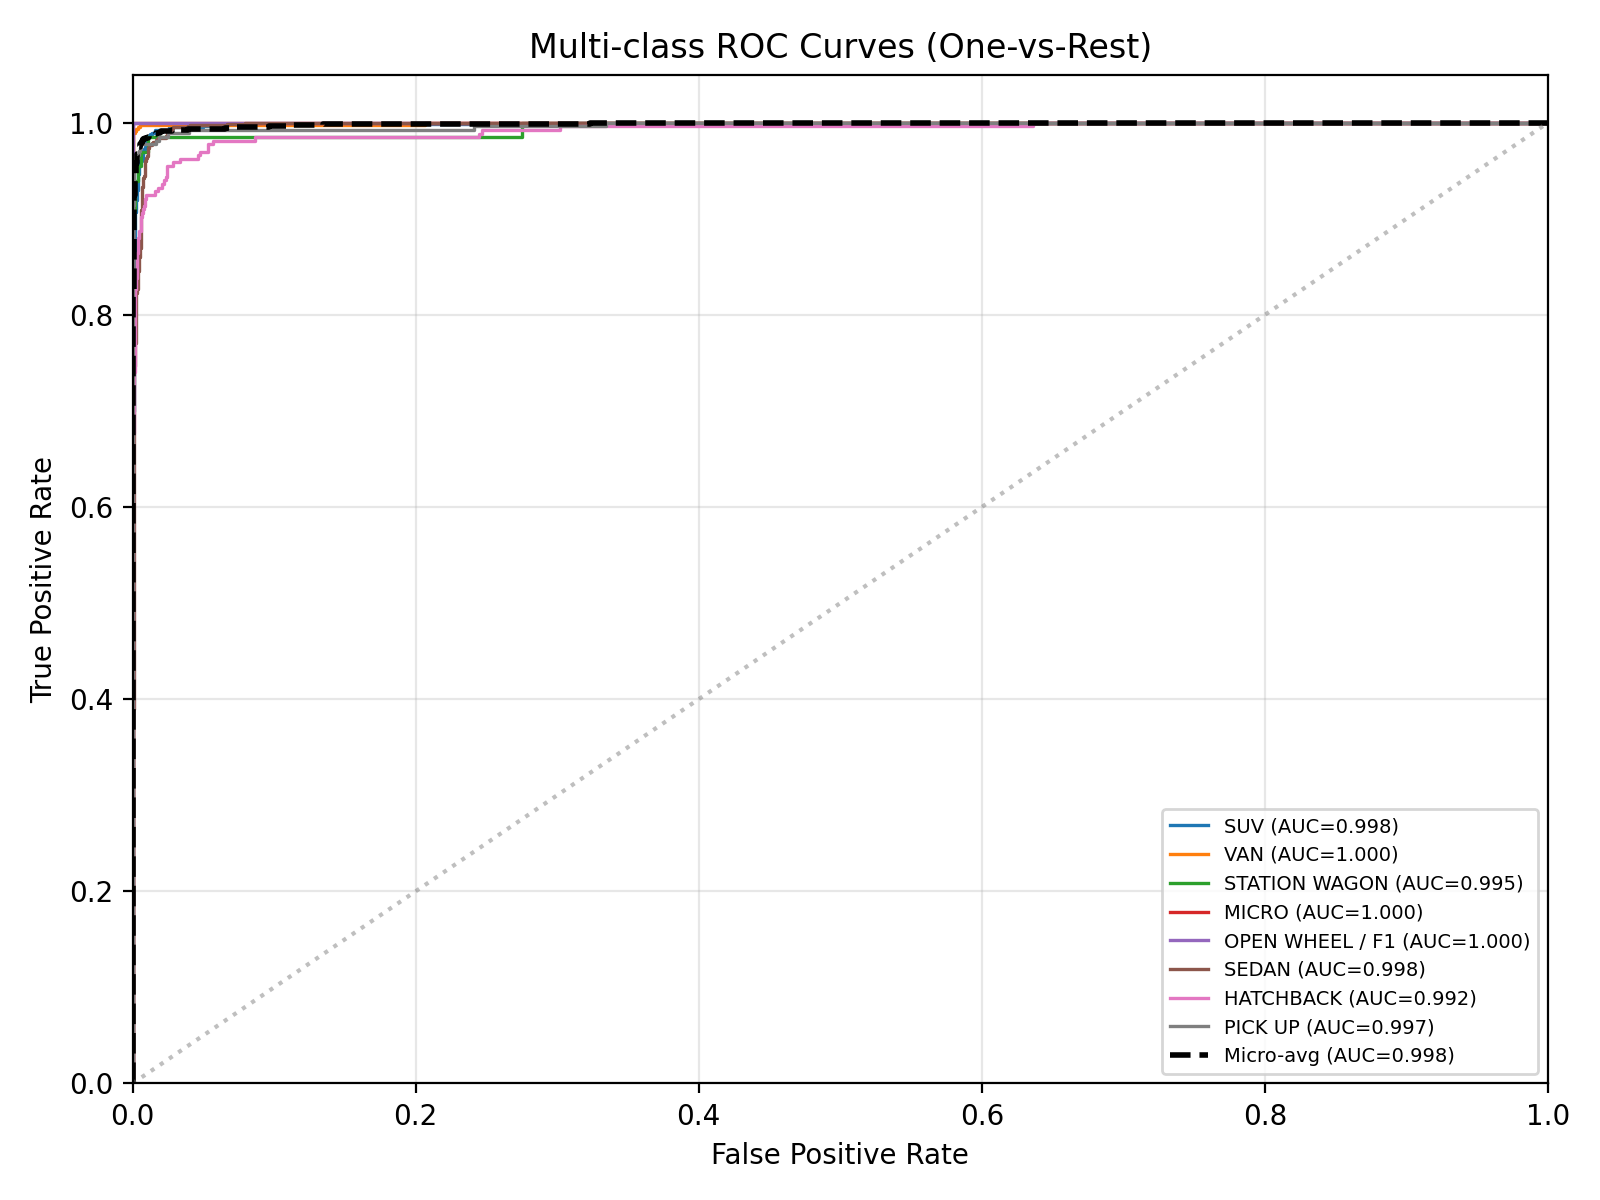
\includegraphics[width=\columnwidth]{images/roc_curves.png}
\caption{İç test seti çok sınıflı ROC eğrileri (One-vs-Rest). Makro OVR AUROC = 0.9975.}
\label{fig:roc}
\end{figure}

Şekil \ref{fig:roc}'de modelin her sınıf için One-vs-Rest ROC eğrileri gösterilmektedir. Her sınıf için [FPR, TPR] ikilisi, modelin softmax olasılıklarının tüm olası eşik değerlerindeki başarımını yansıtmaktadır. Makro OVR AUROC değeri 0.9975 olup, sınıflandırıcının tüm sınıfları mükemmele yakın ayırt edebildiğini göstermektedir. Sınıf bazında en yüksek AUROC değerleri Açık Tekerlekli / F1 (1.0000), Micro (0.9999) ve VAN (0.9995) sınıflarında elde edilmiştir. En düşük AUROC değerine sahip sınıf Hatchback (0.9917) olmasına rağmen, bu değer dahi mükemmel ayrım gücüne işaret etmektedir. Micro OVR AUROC (0.9984), sınıflar arası örnek sayısı farkına rağmen modelin ranking performansının tüm karar eşiklerinde tutarlı olduğunu doğrulamaktadır. Bu sonuçlar, Weighted CE kaybının azınlık sınıflarında yalnızca sınıflandırma doğruluğunu değil, aynı zamanda olasılık sıralamasını da koruduğunu göstermektedir. ROC analizi Dirichlet kalibrasyonu sonrası 3170 iç test örneği kullanılarak gerçekleştirilmiştir.

İç test seti karışıklık matrisi incelendiğinde diyagonal değerlerin yüksek olduğu, en sık hataların Hatchback-Sedan (Hatchback'lerin \%10.2'si Sedan olarak sınıflandırılmış) ve Pick Up-SUV (Pick Up'ların \%7.1'i SUV olarak sınıflandırılmış) arasında gerçekleştiği görülmektedir. Bu hatalar fiziksel benzerlikten kaynaklanmaktadır: Hatchback ve Sedan arasındaki temel fark bagaj bölmesinin uzunluğudur ve önden çekilen görüntülerde bu ayrım zorlaşmaktadır. Benzer şekilde, Pick Up kasasının SUV'den ayrımı da yandan görünümde daha belirgindir.

Test setinde en başarılı sınıflar sırasıyla F1 (1.0000), Micro (1.0000) ve VAN (0.9835) olmuştur. Bu sınıfların birbirinden ve diğer sınıflardan morfolojik olarak belirgin şekilde ayrışması (F1'in açık tekerlek yapısı, VAN'ın kutu formu, Micro'un kompakt boyutu) yüksek başarımı açıklamaktadır. SUV sınıfında 670 örneğe karşılık 0.9492 F1 değeri, büyük örnek sayısına rağmen diğer büyük gövdeli araçlarla (Pick Up, Station Wagon) olan benzerlik nedeniyle nispet düşük kalmıştır.

\subsection{Model Çıkarımı ve Web Arayüzü}
Nihai model PyTorch safetensors (82.4 MB) ve ONNX Runtime (82.6 MB) formatlarına dışa aktarılmıştır \cite{paszke2019pytorch,onnxruntime}. ONNX dönüşümü sırasında modelin hesaplama grafiği optimize edilerek operatörler birleştirilmiş, böylece çıkarım süresi PyTorch'a kıyasla \%12 iyileştirilmiştir. Her iki format da proje teslim şartı olan 95 MB sınırının altındadır; bu nedenle herhangi bir niceleme (quantization) işlemine gerek kalmamıştır.

Gradio tabanlı web arayüzü, görsel yükleme (sürükle-bırak veya manuel seçim), anlık önizleme, tahmin sonucu ve Dirichlet kalibreli olasılık dağılımlarını çubuk grafik (bar chart) olarak göstermektedir \cite{gradio}. Kullanıcı, modelin en yüksek olasılık atadığı sınıfı, ikinci en yüksek olasılığı ve tüm sınıfların güven dağılımını tek ekranda görebilmektedir. Arayüz, yüklenen orijinal görüntüyü tahmin çıktısıyla aynı ekranda göstererek sunum sırasında verilecek yeni test görsellerinin hızlı kontrolünü desteklemektedir. Tahmin çıktısı, değerlendirme sürecinde ihtiyaç duyulan örnek adı ve kategori bilgisini doğrudan verecek biçimde düzenlenmiştir.

M2 Pro üzerinde ONNX Runtime ile ortalama 39.6 ms gecikme süresi (tek örneklik: 44.2 ms) ölçülmüştür. Gerçek zamanlı kullanım için kabul edilebilir bu değer, modelin potansiyel bir REST API servisi olarak da kullanılabileceğini göstermektedir.

\begin{figure}[h]
\centering
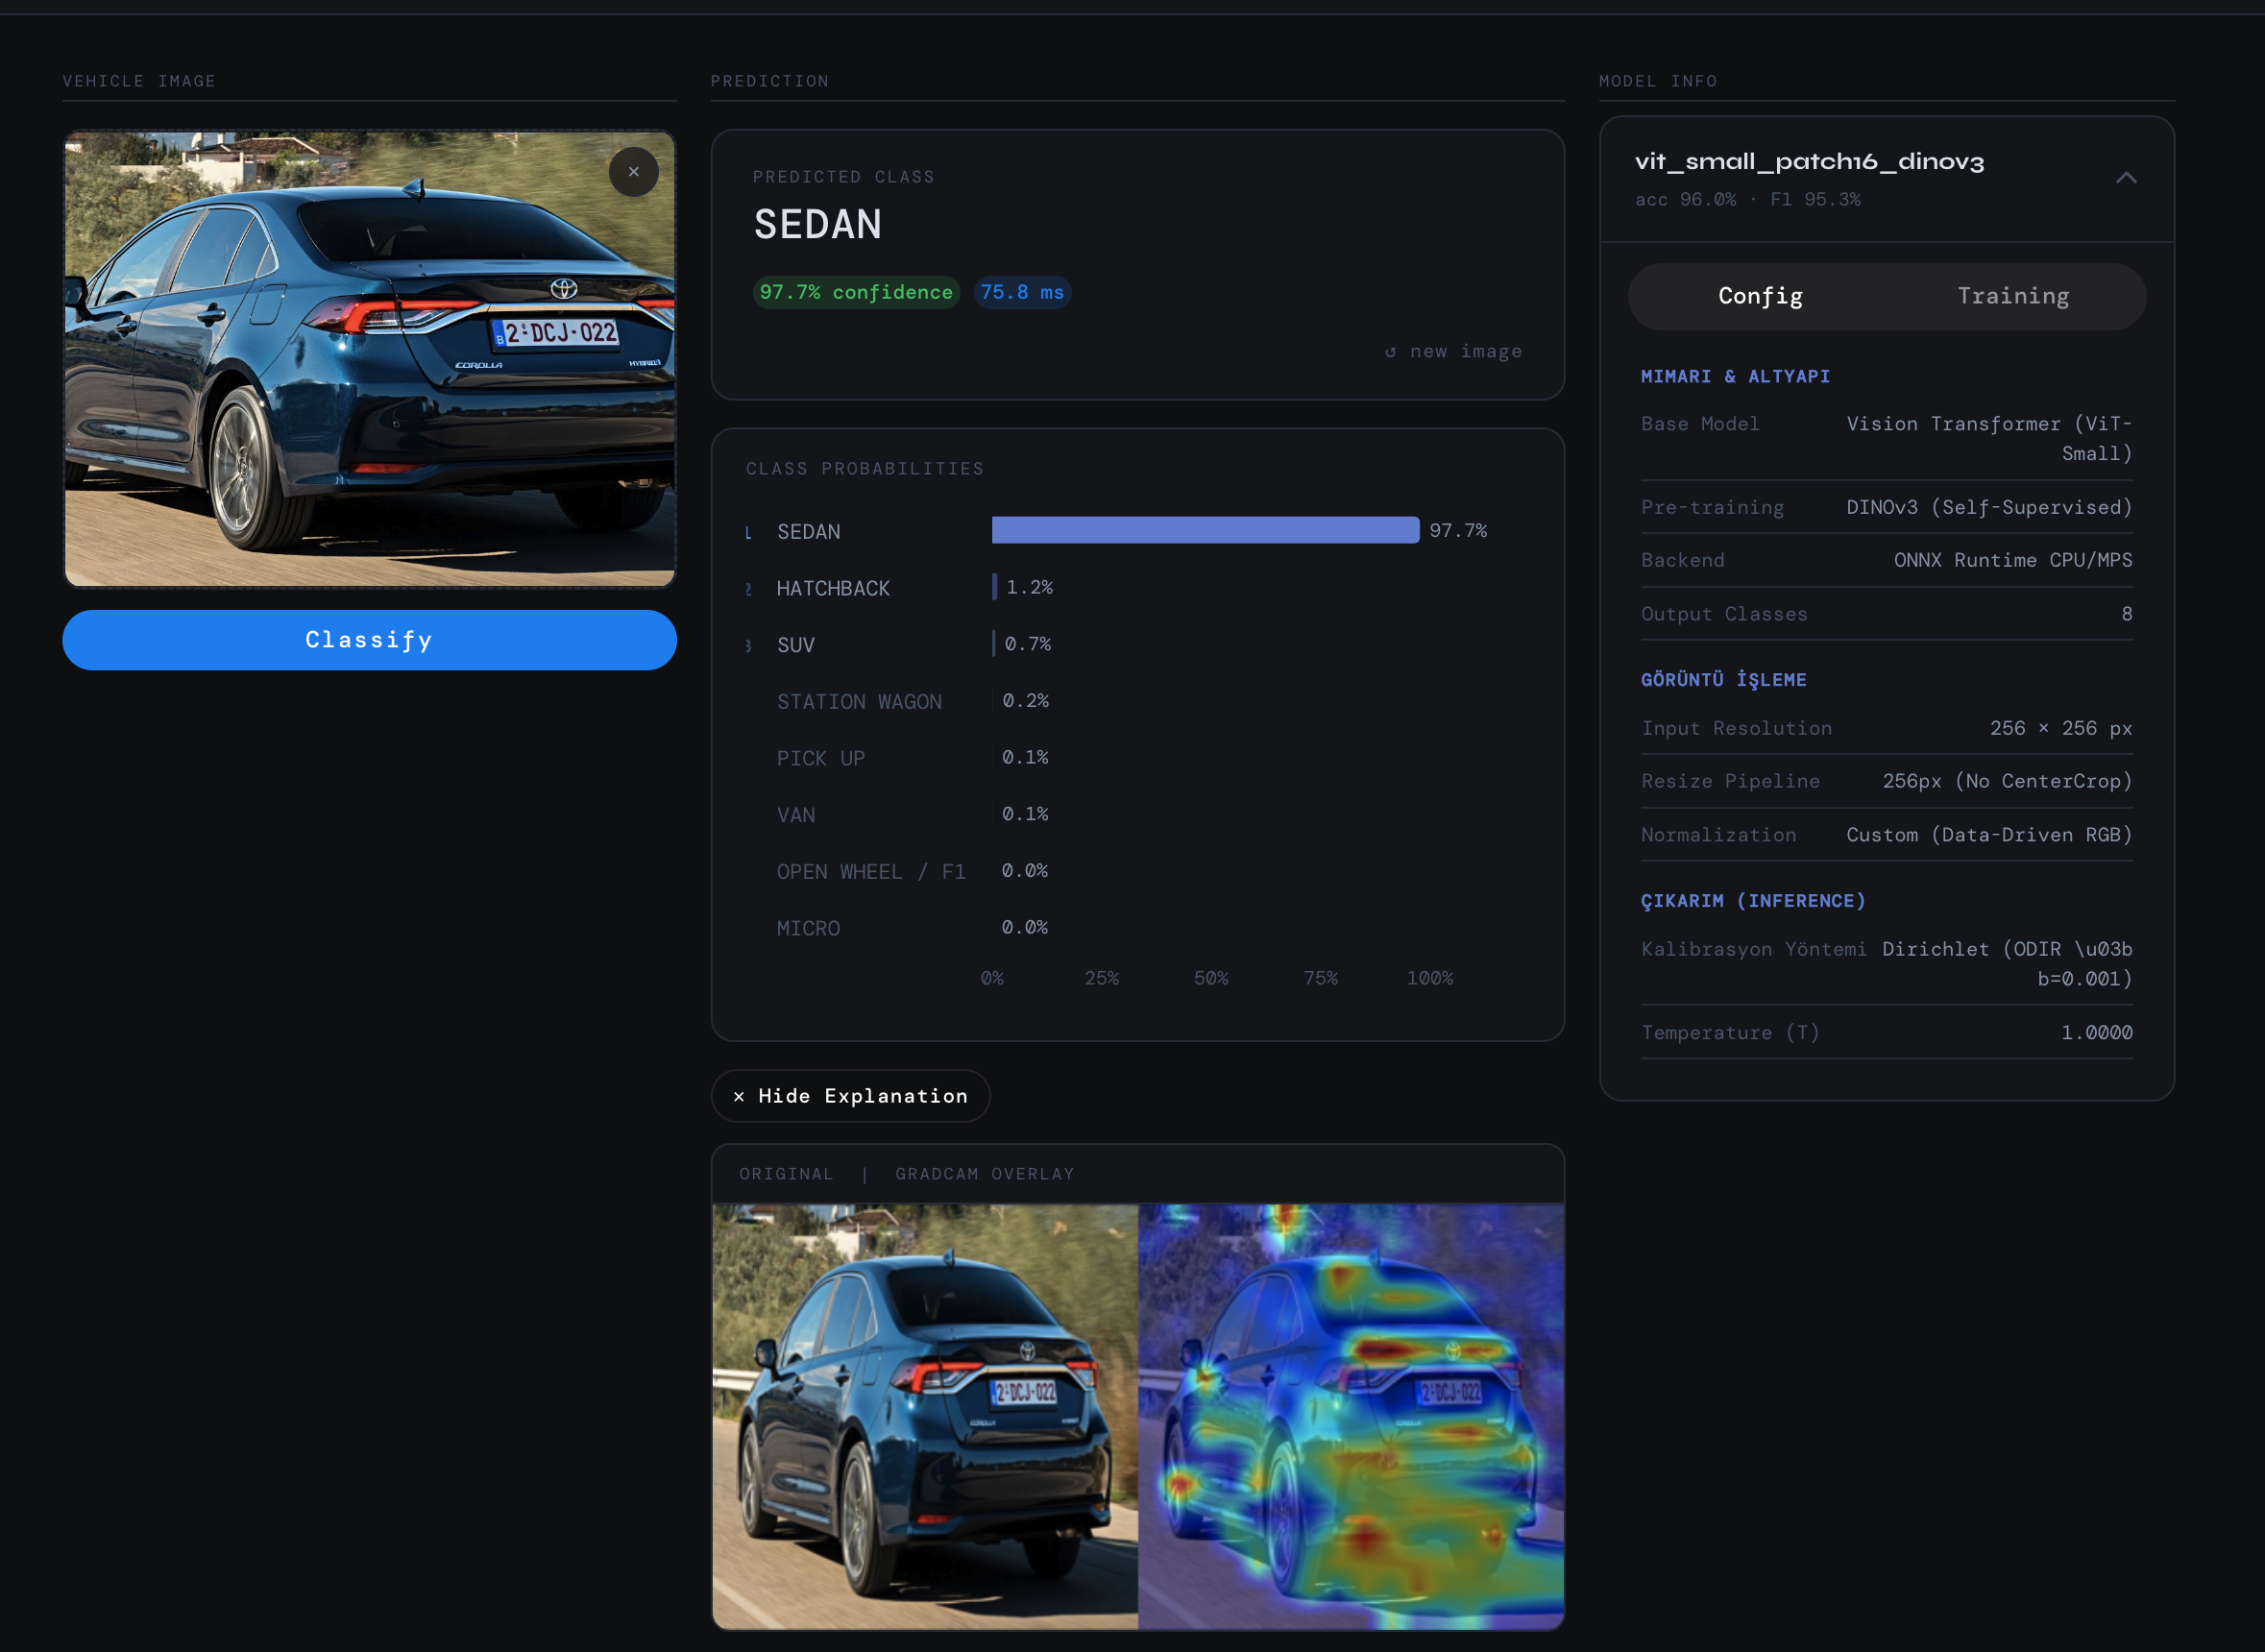
\includegraphics[width=\columnwidth]{images/web_ui.png}
\caption{AutoLens AI web arayüzü kullanıcı ekranı.}
\label{fig:webui}
\end{figure}

\section{Sınırlamalar ve Tartışma}
Mevcut sistemin bazı sınırlılıkları bulunmaktadır:
(1) Veri seti yalnızca açık kaynaklardan toplanmış olup farklı hava/ışık koşullarını, mevsimleri ve coğrafi bölgeleri kapsayan bir dış test seti ile genelleme henüz doğrulanmamıştır. Modelin gerçek dünya performansı, bu tür çeşitlilik içeren bir dış test ile ölçülmelidir.
(2) Hatchback ve Sedan sınıfları arasındaki ayrım, yapısal benzerlik (kısa bagaj, eğimli arka cam) nedeniyle en düşük F1 skoruna (0.8812) sahiptir. Bu iki sınıfın ayrımı için yan/arka profil odaklı ek özniteliklere ihtiyaç duyulmaktadır.
(3) DINOv3'ün daha büyük varyantları (ViT-B/16, ViT-L/14) daha yüksek başarım potansiyeline sahip olmasına rağmen, 95 MB model boyut sınırı nedeniyle denenememiştir. Hali hazırda ViT-S/16 bile 82.4 MB ile bu sınıra oldukça yakındır.
(4) Eğitim yalnızca M2 Pro (MPS) donanımında gerçekleştirilmiş, CUDA/TPU gibi alternatif platformlarda test edilmemiştir. Farklı donanımlarda eğitim dinamiği ve sayısal hassasiyet (BF16 vs FP32) değişebilir.
(5) Focal Loss ablasyonunda $\gamma$ değeri sabit ($\gamma=2.0$) tutulmuş, farklı $\gamma$ değerleri taranmamıştır. Daha düşük $\gamma$ değerleri Weighted CE'ye yakınsayabilir.
(6) Kalibrasyon yöntemleri yalnızca aynı dağılımdaki doğrulama setinde optimize edilmiş olup, dağılım dışı (out-of-distribution) verilerdeki kalibrasyon performansı ölçülmemiştir.
(7) Dirichlet kalibrasyon modeli (8$\times$8 ağırlık matrisi + 8 bias) yalnızca 72 parametre içermesine rağmen, her yeni veri seti için yeniden eğitilmesi gerekmektedir. Temperature Scaling'in tek parametreli yapısına kıyasla bu bir operasyonel dezavantajdır.

Bu sınırlamalara rağmen, sistematik karşılaştırma protokolümüz sayesinde elde edilen bulguların genellenebilir olduğu düşünülmektedir. Özellikle Dirichlet kalibrasyonunun ağırlıklandırılmış kayıp fonksiyonlarından kaynaklanan olasılık bozulmasını düzeltmedeki başarısı, dengesiz veri setleriyle çalışan diğer sınıflandırma problemlerine de ışık tutmaktadır.

\section{Sonuç ve Gelecek Çalışmalar}
Bu çalışmada 8 farklı araba gövde tipini sınıflandıran AutoLens AI sistemi sunulmuştur. Dört farklı mimari (ResNet18, EfficientNet-B2, MobileNetV4, DINOv3 ViT-S/16) aynı veri bölütlemesi ve değerlendirme protokolü altında sistematik olarak karşılaştırılmış, DINOv3'ün öz-denetimli ön eğitim sayesinde CNN tabanlı modellere Makro F1'de +0.0183 ila +0.0682 puan üstünlük sağladığı deneysel olarak gösterilmiştir.

Ablasyon çalışmalarında iki önemli bulgu elde edilmiştir. Birincisi, Weighted Cross-Entropy Loss ile Focal Loss karşılaştırmasında, Weighted CE'nin özellikle azınlık sınıflarında (Micro +0.0465, Station Wagon +0.0650 F1) belirgin iyileşme sağladığı, genel Makro F1'de +0.0205 puan üstünlük kurduğu kanıtlanmıştır. İkincisi, güvenli veri artırımı politikası ve EMA'nın Makro F1'de +0.0320 puan ek iyileşme sağladığı doğrulanmıştır.

Olasılık kalibrasyonu çalışmaları kapsamında üç yöntem karşılaştırılmıştır: Temperature Scaling, Vector Scaling ve Dirichlet (ODIR) kalibrasyonu. Dirichlet yöntemi, Val NLL (0.1371), ECE (\%0.97) ve Test F1 (0.9537) metriklerinde rakiplerini geride bırakmış, modelin aşırı güven sorununu \%90 oranında azaltmıştır. Dört farklı model üzerinde yapılan kalibrasyon analizi, ağırlıklandırma gibi post-hoc düzenlemelerin kalibrasyon ihtiyacını artırdığını ancak Dirichlet yönteminin bu durumda en etkili çözüm olduğunu göstermiştir. Ayrıca $\lambda$ taraması (Tablo \ref{tab:lambda_sweep}), Dirichlet kalibrasyonunun düzenlileştirme parametresine duyarlı olduğunu ve $\lambda=0.001$'in en uygun değer olduğunu ortaya koymuştur.

Nihai model (DINOv3 + Safe Aug + Weighted CE + Dirichlet) \%95.99 doğruluk, 0.9537 Makro F1, 0.9598 Weighted F1 ve 82.6 MB ONNX boyut değerleriyle tüm proje gereksinimlerini karşılamış, Gradio tabanlı web arayüzü ile canlı demo olarak sunulmuştur. Modelin M2 Pro üzerinde ölçülen 39.6 ms gecikme süresi, gerçek zamanlı sınıflandırma senaryoları için uygun olduğunu göstermektedir.

Bu çalışmanın en önemli katkılarından biri, dengesiz veri setlerinde Weighted CE ve Dirichlet kalibrasyonu kombinasyonunun sistematik olarak değerlendirilmesidir. Elde edilen bulgular --özellikle ağırlıklandırmanın olasılık dağılımını bozduğu ancak Dirichlet kalibrasyonunun bu bozulmayı düzeltebildiği yönündeki sonuç-- yalnızca araba gövde tipi sınıflandırması için değil, dengesiz sınıf dağılımına sahip diğer görüntü sınıflandırma problemleri için de yol göstericidir.

Gelecek çalışmalarda Hatchback-Sedan ayrımını güçlendirmek için arka profil ve bagaj yapısına odaklanan ikincil bir sınıflandırıcı geliştirilebilir. Ayrıca modelin genelleme kapasitesi farklı coğrafi bölgelerden toplanmış dış test setleri ile sınanabilir. Model boyutunun izin verdiği ölçüde DINOv3'ün daha büyük varyantlarının (Base) performansı değerlendirilebilir. Son olarak, Focal Loss için hiperparametre taraması ($\gamma$ değerleri) yapılarak daha adil bir karşılaştırma sağlanabilir ve Dirichlet kalibrasyonunun diğer modellerdeki etkisi daha geniş kapsamlı analiz edilebilir.

\bibliographystyle{IEEEtran}
\bibliography{references}

\end{document}
